\documentclass[11pt]{article}
\usepackage{amsthm}
\usepackage{amsmath}
\usepackage{amssymb}
\usepackage{amsfonts}
\usepackage{graphicx}
\usepackage{color}
\usepackage{enumerate}
\usepackage{amscd}

\usepackage{longtable}


\usepackage{algorithm}
\usepackage{algorithmicx}
\usepackage{algpseudocode}

\usepackage[sort&compress,numbers]{natbib}


\usepackage{mathptmx}
%\usepackage[scaled]{helvet}
%\renewcommand\familydefault{\sfdefault}
%\usepackage[T1]{fontenc}





\usepackage{tikz-cd}
\usepackage[hyphens]{url}
\usepackage{wrapfig}
\usepackage{mathrsfs}
\usepackage{mdframed}

\usepackage{dsfont} % blackboard numerals

\usepackage{geometry}
\geometry{margin=0.5in}

\usepackage{setspace}

%\usepackage{endfloat}



\newcommand{\R}{\mathbb{R}}
\newcommand{\E}{\mathbb{E}}
\newcommand{\Econd}{\E_{\Yij|\Yinj,\xinj}}
\newcommand{\EXY}{\E_{\Yinj,\xinj}}
\newcommand{\Prob}{\mathbb{P}}
\newcommand{\LDGP}{L^{\text{DGP}}}
\newcommand{\lDGP}{l^{\text{DGP}}}
\newcommand{\lcox}{l^{\text{Cox}}}
\newcommand{\lpois}{l^{\text{Pois}}}
\newcommand{\hazt}{\lambda_{ij}(t)}
\newcommand{\Yij}{Y_{ij}}
\newcommand{\Yik}{Y_{ik}}
\newcommand{\Yinj}{Y_{i-j}(t)}


\newcommand{\cDE}{\text{\it cDE}}
\newcommand{\mDE}{\text{\it mDE}}
\newcommand{\mPE}{\text{\it mPE}}

\newcommand{\xij}{x_{ij}}
\newcommand{\xik}{x_{ik}}
\newcommand{\xinj}{x_{i-j}}
\newcommand{\tij}{t_{ij}}
\newcommand{\tik}{t_{ik}}
\newcommand{\T}{\mathbf{T}}
\newcommand{\V}{\mathbf{V}}
\newcommand{\W}{\mathbf{W}}
\newcommand{\X}{\mathbf{X}}
\newcommand{\Y}{\mathbf{Y}}
\newcommand{\Z}{\mathbf{Z}}
\newcommand{\bH}{\mathbf{H}}
\newcommand{\h}{\mathbf{h}}
\newcommand{\x}{\mathbf{x}}
\newcommand{\y}{\mathbf{y}}
\newcommand{\z}{\mathbf{z}}
\newcommand{\w}{\mathbf{w}}

\newcommand{\bomega}{\boldsymbol{\omega}}
\newcommand{\bxi}{\boldsymbol{\xi}}
\newcommand{\btheta}{\boldsymbol{\theta}}
\newcommand{\bphi}{\boldsymbol{\phi}}
\newcommand{\balpha}{\boldsymbol{\alpha}}
\newcommand{\betapois}{\hat{\beta}_{\text{Pois}}}
\newcommand{\betacox}{\hat{\beta}_{\text{Cox}}}
\newcommand{\betaDGP}{\hat{\beta}_{\text{DGP}}}
\newcommand{\betaPA}{\hat{\beta}_{\text{PA}}}
\newcommand{\er}{\text{error}}
\newcommand{\omegastar}{\omega^{\textstyle{*}}}
\newcommand{\etastar}{\eta^{\textstyle{*}}}

\newcommand{\dx}[1]{\ \text{d} #1}
\newcommand{\indicator}[1]{\mathds{1}\!\left\{ #1 \right\}}
\newcommand{\indep}{\ \rotatebox[origin=c]{90}{$\models$}\ }
\newcommand{\nindep}{\not\!\perp\!\!\!\perp}

\newcommand{\comment}[1]{[\textcolor{red}{#1}]}

\newtheorem{thm}{Theorem}[section]
\newtheorem{prop}{Proposition}
\newtheorem{cor}{Corollary}
\newtheorem{lem}{Lemma}
\newtheorem{defn}{Definition}

\setlength{\bibsep}{0.0pt}
\setlength{\parskip}{1em}
\setlength{\parindent}{0.0pt}


\allowdisplaybreaks


% Blinding for peer review: set to 1
\newcommand{\blind}{0}



\title{COVID-19 projections for Connecticut: \\ Summer 2020 reopening scenarios}

\author{
  Forrest W. Crawford$^{1,2,3,4}$,
  Olga Morozova$^{1}$, 
  and
  Zehang Richard Li$^1$
  \\[1em]
\small 1. Department of Biostatistics, Yale School of Public Health \\
\small 2. Department of Statistics \& Data Science, Yale University \\
\small 3. Department of Ecology \& Evolutionary Biology, Yale University \\
\small 4. Yale School of Management }



%%%%%%%%%%%%%%%%%%%%%%%%%%%%%%%%%%%%%%%%%%%%%%%%%%%%%%%

\begin{document}

\maketitle

%%%%%%%%%%%%%%%%%%%%%%%%%%%%%%%%%%%%%%%%%%%%%%%%%%%%%%%

\section*{Introduction}

Connecticut is one of the US states most severely impacted by the COVID-19 pandemic, with over 37,000 cases, 11,000 hospitalizations, and 3,400 deaths \citep{nyt2020Connecticut,atlantic2020data}. 
%Most cases and deaths are located in Fairfield, New Haven, and Hartford counties.   
Connecticut began interventions to slow transmission in mid March 2020.  On March XXX, Governor Ned Lamont ordered all in-person classes at K-12 schools cancelled until XXX, and later extended the closure for the remainder of the 2019-2020 academic year.  The Governor issued a statewide ``Stay Safe, Stay Home'' order March 20, to take effect on March 23 [ref].  Evidence from device mobility data suggests that Connecticut residents reduced travel outside the home, and increased the number of hours per day spent at home [mobility refs].  At the same time, the Governor ordered businesses closed, with the exception of essential businesses that could remain open with additional restrictions and guidelines.  Essential businesses included those providing healthcare, infrastructure, manufacturaing, retail, food and agriculture, services, Providers of basic necessities to economically disadvantaged populations, construction, safety, government vendors, and defense were permitted to continue normal operations.  All essential employers were required to implement safe workplace rules to minimize close contact between individuals.  Retail businesses were permitted to remain open under ``Safe Store Rules''. Food service businesses were permitted to offer take-out or delivery services only. Gyms, theaters, hair and nail salons, barbershops, spas, and tattoo parlors were ordered closed.  COVID-19 hospital census peaked in mid April and began a slow decline through April and into May.   


% Reopening plans

On May 8, Governor Lamont issued plans and guidance for reopening the state, a process scheduled to begin on May 20.  The Connecticut Department of Economic and Community Development issued rules and guidelines for opening particular business sectors \citep{decd2020coronavirus}. Summer camps will be permitted to open effective June 29, 2020 subject to restrictions on operations.  Connecticut's Shorline State Park beaches will reopen on Memorial Day weekend under restrictions on the size of gatherings, proximity, and face coverings \citep{ct2020parks}.  Contact tracing will be implemented using the \emph{ContaCT} platform \citep{ct2020contact}.  The state plans to scale up COVID-19 PCR testing [ref], but testing capacity is still limited \cite{thomas2020surge}. The state publishes daily testing reports \citep[e.g.][]{ct2020testing}. 



% summary: 

In this report, we use a mathematical infectious disease transmission model to project COVID-19 incidence, prevalence, hospitalizations, and deaths in the state of Connecticut through August 31, 2020.  We consider population-level contact scenarios informed by the Connecticut Governor's phased reopening plans.  Model parameters are calibrated using data on hospitalizations and deaths in Connecticut and estimates from the literature on clinical epidemiology of SARS-COVID-19.  A separate technical report describes the data, transmission model, and calibration in detail \citep{morozova2020tech}.  The primary purpose of this report is to provide state and local decision-makers with information to plan reopening of the state in a way that minimizes the risk of a resurgence in COVID-19 cases, hospitalizations, and deaths.  The secondary purpose is to assist state agencies and non-governmental organizations in implementation of public health responses, including testing, contact tracing, and design of incidence, infection prevalence, and seroprevalence studies. 




%%%%%%%%%%%%%%%%%%%%%%%%%%%

\section*{COVID-19 projections} 

We present projections of COVID-19 incidence, prevalence, hospitalizations, and deaths from March 1 to August 31.  Projections prior to \today are calibrated to historical hospitalization and death data obtained from [data sources].  Projections beyond \today depend on assumptions about the nature of contact and viral testing in the future, under the Governor's plan for reopening the state.  Projections and 90\% uncertainty intervals show the range of possible outcomes over the summer in under ``slow'' and ``fast'' reopening scenarios.  

A separate technical report describes the data, transmission model, calibration, and uncertainty calculation in greater detail \citep{morozova2020tech}.  Briefly, we employ a modified susceptible-exposed-infectious-removed (SEIR) transmission model that accommodates asymptomatic, mildly symptomatic, and severe cases, hospitalizations, and deaths.  

[Briefly discuss lagging hospitalizations and deaths to match reporting.]


\subsection*{Calibration and fit to historical data}


Figure \ref{fig:calibration} shows...

% \comment{Richard, could you create a figure showing model fit to data for hospitalizations and deaths?}


\begin{figure}
\centering
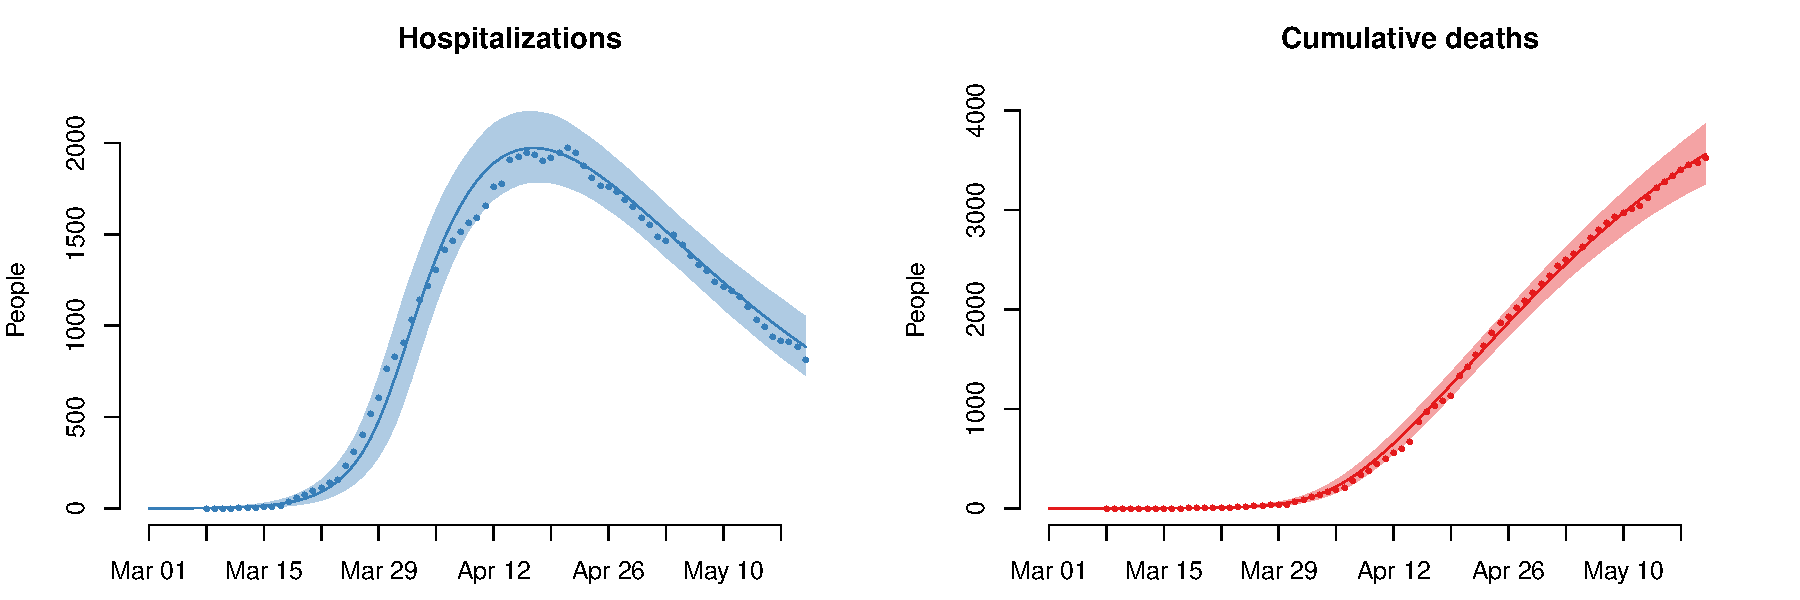
\includegraphics[width=.9\textwidth]{figures/calibration.pdf}
\caption{Illustration of model fit to COVID-19 hospitalization and death data in Connecticut. }
\label{fig:calibration}
\end{figure}


\subsection*{Summer projections under slow reopening} 




\subsection*{Summer projections under fast reopening} 




%%%%%%%%%%%%%%%%%%%%%%%%%%%%%%%%%%%%


\section*{Implications}

The COVID-19 outbreak in Connecticut is currently declining, with hospitalization census and the number of deaths per day decreasing since mid April  However, as the state reopens, there is a risk that increased contact will result in a surge of COVID-19 transmission, leading to an increase in hospitalizations and deaths. 


\subsection*{Risk of resurgence following reopening} 

Projections under high asymptomatic fraction or fast reopening suggest that increased transmission following reopening may result in a rapid rise in hospitalization during August, with an increase in deaths following soon after.  It is important to note that if transmission increases immediately following reopening, the first indications of this increase would not be apparent until mid to late July, as the first post-reopen infections become hospitalizations.  Therefore it is important that public health authorities closely monitor new hospitalizations as well as hospital census for signs of increased numbers COVID-19 cases requiring healthcare.  


\subsection*{Importance of testing to detect changes in incidence}

Enhanced viral testing, especially of asymptomatic individuals, may help provide an early warning of increased transmission following reopening.  Because there is a roughly 3-week lag between increased incidence and increased hospitalization, widespread and frequent testing could detect increased incidence before the first new symptomatic cases present to the hospital. 

Daily new infections are not observable, but can be estimated...

[show daily incidence plots]


\begin{figure}
\centering
% \includegraphics...
\caption{\comment{show daily incidence}}
\label{fig:cumincidence}
\end{figure}

Figure \ref{fig:cumincidence} 



\subsection*{Epidemiological study design}

Expanded antibody testing in Connecticut could dramatically increase certainty about seroprevalence -- the number of people who have evidence of prior infection. If this proportion were more precisely known, the fraction of infected individuals who are asymptomatic could be estimated with greater certainty.  This knowledge would reduce uncertainty in future projections.  
sample size calculations for seroprevalence study


\begin{figure}
\centering
% \includegraphics...
\caption{\comment{show cumulative alive incidence and current prevalence }}
\label{fig:cumincidence}
\end{figure}

Figure \ref{fig:cumincidence} shows cumulative incidence among individuals currently alive....



\subsection*{Uncertainty about child care, summer camp, and school reopening}

Epidemiologists do not yet know how transmissible school-age children may be ... conflicting evidence of viral shedding and transmissibility. 

\comment{Olya, can you write a few sentences and give references for what we know and don't know about transmission in children?}

Because the state closed K-12 schools approximately one week before the stay-at-home order was implemented, we do not have specific information about the effect of closing schools on reduction in transmission.  If child care and summer camps reopen as planned [ref] in early July, we may gain information about the possible effect of school reopening in the Fall.  


%%%%%%%%%%%%%%%%%%%%%%%%%%%

\textbf{About this report}: The most recent version of this report is available from [Project web page] with source at \url{https://github.com/fcrawford/covid19_ct_report1}. Release versions are hosted at \url{https://github.com/fcrawford/covid19_ct_report1/releases}. 


%%%%%%%%%%%%%%%%%%%%%%%%5

\textbf{Disclosures}: FWC is a member of the Reopen Connecticut Steering Committee.  The authors report no conflicts of interest. 

%%%%%%%%%%%%%%%%%%%%%%%%5


\textbf{Acknowledgements}:
Matthew Cartter,
Joshua Geballe,
Gregg S. Gonsalves,
Alexander Karnal,
Albert Ko 



%%%%%%%%%%%%%%%%%%%%%%%%%%%%%

\bibliographystyle{unsrtnat}
\bibliography{covid19}


\end{document}

